\subsection{Complementary Attack}

This attack is carried out adding an extra function to the \code{controller}
FMUs. The attack consists into changing the values coming from sensors with
their complement (\(255 - value\)). This implies that instead of white the
controller sees black and vice-versa (with the exclusion of some readings near
to the colour threshold).

\lstinputlisting[language=C, label={lst:complementary_attack},
caption={Attack algorithm.}]{complementary_attack_ctrl.c}

The attack function for sensors must be placed at the beginning of the regular
controller \code{tick} function.

\begin{figure}[htb]
	\centering
	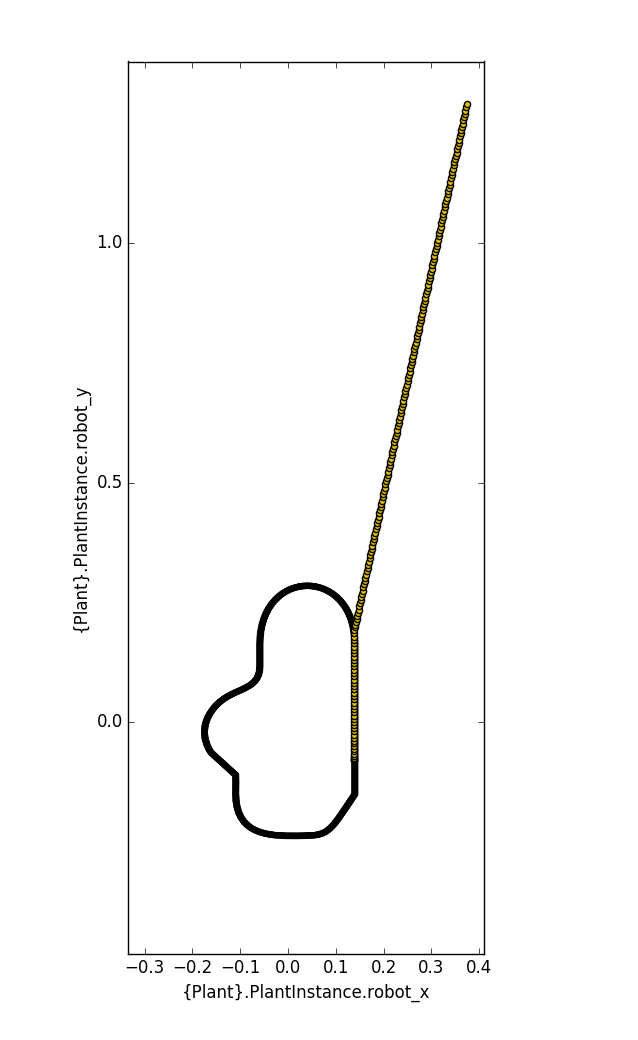
\includegraphics[width=0.5\textwidth]{complementary-attack}
	\caption{Line follower robot path when
	attacked}\label{fig:complatkresult}
\end{figure}

We can see from \figref{fig:complatkresult} that instead of turning left the
robot turns right. It is correct because sensor values are complemented, so the
consequent speed of the wheel is inverted between the two wheels.
